\chapter{Gjennomføring av forsøk}\label{chap:gjennomforing}
Får å kunne svare på forskningsspørsmålet og validere hypotesene, jf. delkapittel~\ref{sec:forskningssporsmaal}, ble det gjennomført et eksperiment bestående av forsøk både på pakningsvedlegg og på Mine Medisiner. Eksperimentet fokuserte på tid, kunnskap og korrekthet. Brukbarheten til både pakningsvedlegg og Mine Medisiner ble også målt. I dette kapittelet vil utviklingen av eksperimentet, gjennomføring av forsøkene, deltakergruppen og planen for analysen av resultatene bli presentert.



\section{Utvikling av eksperimentet}
Vi bestemte oss for å gjennomføre en prøvegjennomføring av eksperimentet vi lagde. Under prøvegjennomføringen av eksperimentet fant vi noen svakheter som gjorde at vi endret eksperimentet. 

I prøvegjennomføringen hadde vi åpne spørsmål uten svaralternativer. Vi oppdaget at det var dumt at vi ikke benytte oss av svaralternativer. Ved bruk av svaralternativer ville det vært enklere å avgjøre hva som var riktige og gale svar. Dette ville gjort det lettere å sammenligne to deltakere, og å analysere resultatene. Vi fant ut at istedenfor å ha spørsmål med svaralternativer kunne det være lurt med utsagn som deltakerene vurderer hvor enig de er i. Ved å bruke en slik skala kunne vi bedre måle styrken på holdninger og opplevelser som deltakergruppen hadde. 

Prøvegjennomføringen viste at forsøket tok alt for lang tid å gjennomføre. For å korte ned tiden på forsøket gjorde vi utsagnene mer konkrete og presise. Et eksempel er at istedenfor å spørre om “Hvilke av dine legemidler har interaksjoner?” ba vi deltakerene om å vurdere utsagnet “Jeg bør ikke ta Albyl-E og Ibux.”. Dette gjorde at deltakerene ikke trengte å sjekke alle legemidlene.

En annen god effekt ved å spørre mer konkrete og presise utsagn var at pasienter som leser pakningsvedlegg eller andre kilder antagelig oftere leter etter informasjon som kan gi besvare konkrete spørsmål enn generell informasjon. Vi anså derfor det som bedre at deltakerene skal vurdere utsagnet “Jeg har hodepine fordi jeg har tatt Albyl-E.” enn at de skulle svare på “Hvilke av dine legemidler kan gi hodepine?”.

I spørsmålene i prøvegjennomføringen brukte vi ordet \textit{interaksjon}. Vi oppdaget at deltakerne ikke forstod dette ordet. Utsagnene vi formulerte til de ordentlige forsøkene inneholder derfor ikke ordet \textit{interaksjon}, men heller en lenger forklaring av hva en interaksjon er. 

Under prøvegjennomføringen valgte vi å la den samme deltakeren utføre de samme oppgavene både på pakningsvedlegg og Mine Medisiner. Årsaken til dette var fordi vi mente at det ville gjøre det enklere å sammenligne systemene. Vi oppdaget at deltakerene benyttet seg av svarene de fant ved å bruke det første systemet når de skulle finne svarene med det andre systemet. Dette gjorde det vanskeligerer å sammenligne systemene, og vi bestemte oss derfor for å at utsagnene skulel vurderes ved hjelp av et system per deltaker. Ved at deltakeren kun benytter seg av et system i et forsøk vil forsøket gå raskere, noe som var ønskelig. 

\section{Rekruttering av deltakere}
Vi ønsket å rekrutere mellom 10 og 15 \acrshort{tia}\footnote{TIA: hjerneslag hvor symptomene trekker seg tilbake i løpet av 24 timer}-pasiener til forsøkene våre. Vi tok kontakt med flere ansatte ved St. Olav universitetssykehus for å få hjelp til å rekrutere \acrshort{tia}-pasiener til forsøkene. Vi tok kontakt med både farmasøyter ansatt på sykehusapoteket og leger ansatt ved slagavdelingen. Etter flere uker med frem og tilbake måtte vi innse at det var for tidkrevende å skulle rekrutere 10-15 deltakere som har hatt \acrshort{tia}. Det var også for vanskelig å rekrutere andre pasientgrupper fra sykehuset. Vi valgte derfor å rekrutere deltakere gjennom vårt sosiale nettverk. Dette gjorde at demografien til deltakergruppen ble ganske annerledes fra det vi så for oss i utgangspunktet. 

Deltakerene ble valgt ut tilfeldig blant bekjente som hadde tid og anledning til å delta, og besto totalt av 13 personer. 6 deltakere utførte forsøk på Mine Medisiner og 7 deltakere utførte forsøk på pakningsvedlegg.
    
\section{Oppbygging av forsøket}
Forsøket besto av syv deler, se vedlegg~\ref{chap:utforming}.

Den første delen av forsøket var en introduksjon hvor deltakere ble informert om forsøket formål og utforming. deltakerene gav skriftlig samtykke til å delta i forsøket ved å signere samtykkeskjema, se vedlegg~\ref{chap:samtykke}. Skjemaet informerte om at indirekte personopplysninger vil bli slettet eller endret slik at de ikke er personidentifiserende, etter prosjektets slutt. Detaljer fra gjennomføringen av hver enkelt forsøk er ikke gjengitt i rapporten.

I forsøkets andre del ble demografiske opplysninger om deltakerne samlet inn ved at deltakeren svarte på et skjema med spørsmål om alder, yrke, utdanning, datakunnskap og legemiddelbruk, se vedlegg~\ref{chap:demografi}. De demografiske opplysningene ble samlet for å kunne bli brukt til å analysere resultatene.

Den tredje delen av forsøket besto av spørsmål om deltakeres forkunnskap om legemidler. 

Den fjerde delen, hoveddelen av forsøket, besto av syv utsagn deltakere skulle ta stilling til, se vedlegg~\ref{chap:paastander}. Utsagnene \todo{presenter utsagnenes innhold}. 
Utsagnene skulle vurderes ved hjelp av Mine Medisiner eller pakningsvedlegg. Deltakerne fikk utdelt en tekstlig beskrivelse av Håkon, se vedlegg~\ref{chap:haakon}, og ble bedt om å ta stilling til utsagnene som om de var Håkon. Den totale tiden det tok å ta stilling til de syv utsagnene ble målt for hvert forsøk. Etter at alle utsagnene var vurdert ble deltakerne bedt om å forklare årsakene til at de vurderte utsagnene som de gjorde. Ved å vente med å be om forklaringene til etter alle utsagnene var vurdert forstyrret vi deltakerene i minst mulig grad mens de vurderte utsagnene.

Den femte delen av forsøket besto av en rekke spørsmål for å sjekke om deltakeren lærte noe ved å bruke systemet, se vedlegg~\ref{chap:utforming}. Spørsmålene skulle besvares uten hjelpemidler. Noen av spørsmålene var relatert til utsagnene i del tre. Andre spørsmål var ikke eksplisitt knyttet til utsagnene, men kun til legemiddellisten generelt. Hensikten var å finne ut hvor mye deltakeren husket fra det de ble spurt om i del tre, og å finne ut hvor mye deltakerene lærte utover det som eksplisitt ble spurt om i del tre. 

I den sjette delen av forsøket fylte deltakeren ut et \acrshort{sus}-skjema for systemet de benyttet seg av under forsøket. Spørsmål 4 fra det originale \acrshort{sus}-skjemaet var endret til: “jeg vil måtte trenge hjelp fra en person med faglig kunnskap for å kunne bruke systemet”, fordi teknisk kunnskap ikke er relevant for pakningsvedlegg. Vår tolkning er at faglig kunnskap kan bety helsepersonell og teknisk personell for Mine Medisiner, og kun helsepersonell for pakningsvedlegg. Se vedlegg~\ref{chap:SUSPak} for \acrshort{sus}-skjema for pakningsvedlegg, og vedlegg~\ref{chap:SUSMM} for \acrshort{sus}-skjema for Mine medisiner.

I den syvende delen av forsøket skulle deltakeren velge 5 av 39 ord som de mente best beskrev systemet de benyttet seg av under forsøket, se tabell~\ref{tab:reactionCardTabVedlegg} i vedlegg~\ref{chap:utforming}. Etterpå skulle de begrunne valget av ord.


\section{Analyse}
Analysen av resultatene vil ta utgangspunkt i hypotesene fra delkapittel~\ref{sec:forskningssporsmaal}. Hoveddelen av analysen vil derfor gå ut på å sammenligne de to systemene. Det er vanskelig å forutse resultatene fra forsøkene. Vi antar derfor at deler av analysen ikke kan planlegges. Under presenteres den planlagte analysen, med forbehold om at resultatene vi finner ved analysen vil gi oss resultater vi kan jobbe videre med.  

\subsection{Demografi}
Demografien for forsøkene vil bli sammenlignet for å se om deltakergruppene er like. Hvis deltakergruppene er for ulike vil det være vanskelig å si noe om sammenligningsgrunnlaget for resten av observasjonene. Demografien vil også bli brukt til å prøve å validere resultatene. 

\subsection{Vurdering av utsagn}
Utsagnene har en fasit. Fasiten er utarbeidet basert på informasjon vi har funnet i pakningsvedlegg og etter samtale med farmasøyt. Vurderingsvalget og forklaringen deltakerne gir på utsagnene vil være det som vurderes mot fasiten. Altså kan det skje at``litt enig'' og en god forklaring også gir et blir godkjent som riktig, selv om vi fasiten er at ``enig'' er det riktige valget.

Tiden som ble målt når deltakerne vurderte utsagnene vil bli brukt til å si noe om hvilket system som er raskest å bruke. De demografiske forskjellene på deltakerene må tas høyde for når tidsbruken blir vurdert. 

Å tenke høyt er en mye brukt teknikk under brukertesting. Vi valgte å ikke be deltakeren tenkte høyt, da teorien var at dette ville påvirke tidtakingen. I stedet observerte vi hva deltakeren gjorde underveis, og ba om forklaring i etterkant. Forklaringen bar noen ganger preg av at deltakeren ikke husket nøyaktig hvorfor han vurderte som han gjorde. Dette kunne blitt løst ved å spørre om forklaring umiddelbart etter hvert utsagn. Dette mener vi ville gjort situasjonen kunstig, og det ville påvirket arbeidsflyten til deltakeren. 

\subsection{Læringsutbytte}
Det vil bli undersøkt om deltakeren har klart å tilegne seg kunnskap både i form av å gjengi informasjon de brukte til å vurdere utsagnene og i form av å tilegne seg kunnskap utover dette.

Vi vil bruke et poengsystem med en maks poengsum for å vurdere læringsutbytte. Det er totalt seks spørsmål som sjekket deltakerenes læringsutbytte. Det er bare tre av utsagnene det er mulig å vurdere ved å gjengi informasjon som ble benyttet i utsagnene. De kan maks gis tre poeng for gjengitt informasjon og maks seks poeng for ny informasjon. Man kan altså maks få et poeng for lært informasjon per spørsmål. Deltakeren får altså ikke flere poeng for å vise at de har lært mye på ett spørsmål.

Når en deltakerens poeng for læringsutbytte blir regnet ut vil det tas høyde for hva deltakeren kunne i forkant. Hvis en deltakerer på forhånd oppgir informasjon som også oppgis i læringsutbytte spørsmålene ansees dette som 0 poeng. Hvis deltakeren klarer å gi mer informasjon enn det han på forhånd oppgav vil han få poeng ut i fra poengsystemet i avsnittet over.

Etter alle poengene er regnet ut vil poengene fra Mine Medisiner forsøkene bli sammenlignet med poengene fra pakningsvedlegg forsøkene.

\subsection{System usability scale} \label{subsec:SUS}
\acrfull{sus} vil bli brukt til å analysere systemenes brukbarhet. \acrshort{sus} er en brukbarhetsskala for å gi en subjektiv vurdering av brukbarhet \citep{sus}. Skjemaet inneholder 10 utsagn med tilhørende likert skala fra 1 til 5. Skalaen går fra sterkt uenig til sterkt enig.

Ut i fra \acrshort{sus} skjemaene er det mulig å regne ut en \acrshort{sus} poengsum. Denne poengsummen er et nummer mellom 0 og 100 som representerer et mål på den brukbarheten til systemet.

\acrshort{sus} poengsummen regnes ut på følgende måte:
\begin{enumerate}
\item Alle utsagn får en poengsum basert på skalaen. Velger noen ``sterkt'' uenig på et utsagn vil poenget for dette utsagnet altså bli 1.
\begin{enumerate}
\item For alle utsagnene nummerert med et oddetall skal utsagnets poeng subtraheres med 1.
\item For alle utsagnene nummerert med et partall skal 5 subtraheres med utsagnets poeng.
\end{enumerate}
\item Summer poengene fra alle utsagnene.
\item Ta summen av poengene og multipliser med 2,5. 
\item Resultatet blir en \acrshort{sus} poengsum mellom 0 og 100.
\end{enumerate}

\begin{figure}[H]
    \centering
    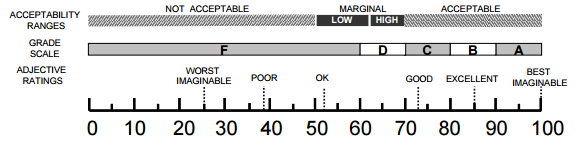
\includegraphics[width=1\textwidth]{fig/eksperimentdesign/sus-score.PNG}
    \caption{SUS karakterskala for å fastslå betydningen av en \acrshort{sus} poengsum \citep{bangor2009determining}}
    \label{fig:sus}
\end{figure}

Bangor et al.\citep{bangor2009determining} har foreslått en karakterskala for å fastslå betydningen av \acrshort{sus}-poengsummen, se figur~\ref{fig:sus}. I følge denne karakterskalaen er et system med en \acrshort{sus}-poengsum på over 70 et brukbart system, et system med en poengsum på 75-85 er et bedre system og et system med en poengsum på over 85 er et utmerket system. Denne karakterskalaen vil bli brukt i analysen av resultatene av forsøkene. Denne skalaene vil bli brukt for å vurdere brukbarheten til pakningsvedleggene og Mine Medisiner. 

\subsection{Reaction cards} \label{sec:reactionCards}
Reaction cards er en måte å få frem negative og positive meninger fra deltakeren om deres meninger om systemet, samt skape diskusjon mellom observerer og deltaker. Reaction cards er et sett med 118 ord som benyttes til diskusjon av systemer ved brukbarhetstesting. I dette eksperimentet ble bare 39 av disse ordene benyttet. Ordene som ble valgt ut var de vi anså som mest aktuelle for de to systemene, og den sammenligningen vi skal gjøre. En mulig feilkilde til resultatene er at vi har valgt ut for mye av samme typen ord. Det at deltakerene ofte gir positive tilbakemeldinger etter brukertester er også en mulig feilkilde \citep{MeasuringSatisfaction, MeasuringDesirability}. For å motvirke dette sørget vi for at minst 40\% av ordene var negativt ladet.

Ved analyse av reaction card-delen av forsøket vil frekvensen av ordene vil bli beregnet og sammelignet for de to systemene.    



\clearpage